\newpage

\section{ Design } 
\subsection{ Wireframing}

Wireframing ist ein wichtiger Schritt im Designprozess, bei dem eine grundlegende, schematische Darstellung 
einer Website, einer App oder eines Produkts erstellt wird. Es handelt sich um eine visuelle Skizze, die die 
Struktur, das Layout und die Platzierung von Elementen zeigt, ohne sich auf Details wie Farben oder Schriftarten 
zu konzentrieren.

Aspekte des Wireframings lauten:

\begin{itemize}
    \item Struktur und Layout: Ein Wireframe legt fest, wo sich Hauptelemente wie Header, Navigation, Inhalt und Fußzeile befinden. Es hilft, die Hierarchie der Informationen zu planen.
    \item Funktionalität: Wireframes zeigen, wie Nutzer mit der Anwendung interagieren können. Welche Schaltflächen, Links oder Formulare sind vorhanden?
    \item Inhaltsplatzierung: Es wird festgelegt, wo Texte, Bilder und andere Inhalte platziert werden. Dies hilft, den verfügbaren Platz zu visualisieren.
    \item Feedback und Iteration: Wireframes sind flexibel und können leicht überarbeitet werden. Sie dienen als Diskussionsgrundlage für das Designteam und die Stakeholder.
\end{itemize}

Wireframes können auf Papier, digitalen Tools oder speziellen Wireframing-Softwareanwendungen erstellt werden. Sie sind ein wichtiger erster Schritt,um die 
Benutzeroberfläche zu planen, bevor das eigentliche Design beginnt.

Im Folgenden sehen wir 3 Wireframes des Projekts. Die Umfassen die Landing Page, die Blogpage und ein Blog Eintrag. Die Abbildung \ref*{fig:Landing_Page}
zeigt den Aufbau und Struktur der Seite die ein Besucher der Application als erstes zusehen bekommt.
\begin{figure}[H]
    \caption{Wireframe der Landing Page}\label{fig:Landing_Page}
    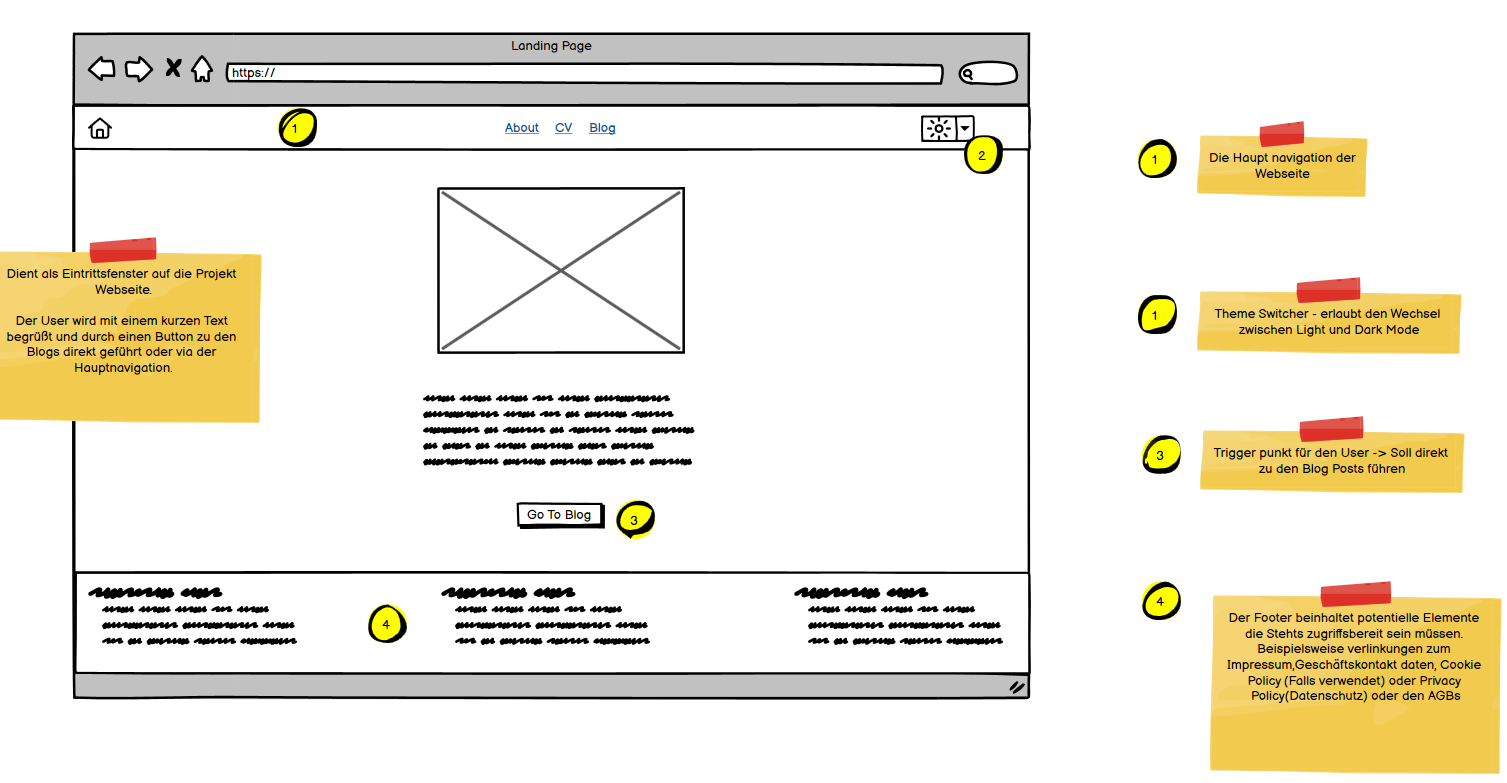
\includegraphics[width=0.5\textwidth]{landingpage.png}
    \\
    Quelle: Eigene Darstellung
\end{figure}

Die Abbildung \ref*{fig:BlogPage} visualisert wie eine kollektion von Blog Einträgen dem Besucher dargestellt werden.

\begin{figure}[H]
    \caption{Wireframe der Blog Page}\label{fig:BlogPage}
    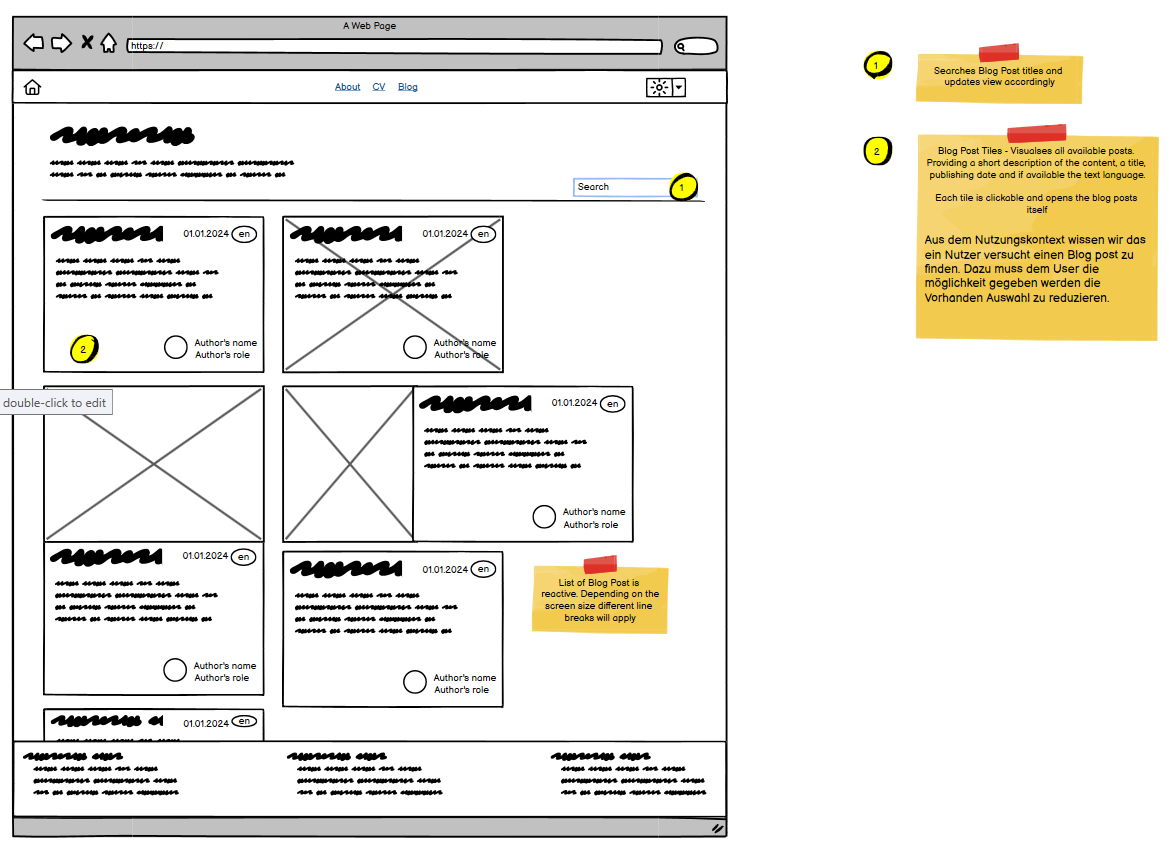
\includegraphics[width=0.5\textwidth]{blogpage.png}
    \\
    Quelle: Eigene Darstellung
\end{figure}

Und das letzte Wireframe die Abbildung \ref*{fig:BlogEntry} Zeigt wie ein einzelner Blog Eintrag dem Besucher visualisert wird.
\begin{figure}[H]
    \caption{Wireframe eines Blog Eintrags}\label{fig:BlogEntry}
    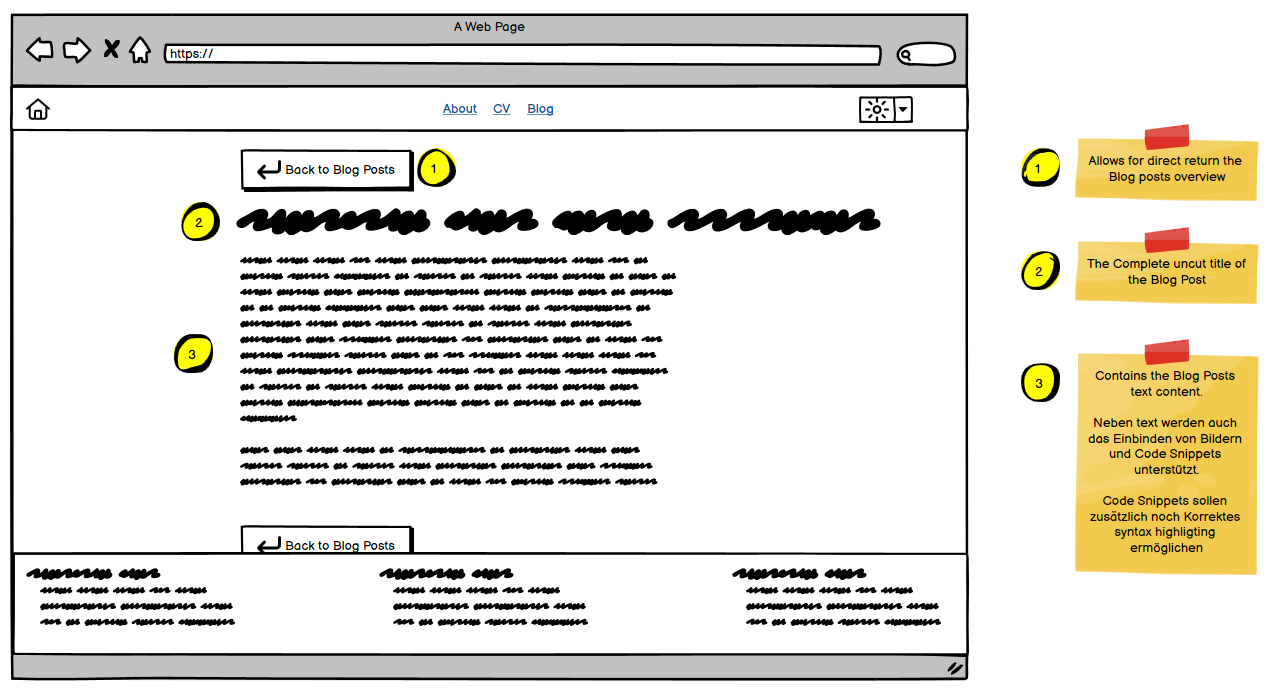
\includegraphics[width=0.5\textwidth]{blogentry.png}
    \\
    Quelle: Eigene Darstellung
\end{figure}
 
\subsection{ Sitemap }

\begin{figure}[H]
    \caption{Sitemap}\label{fig:Sitemap}
    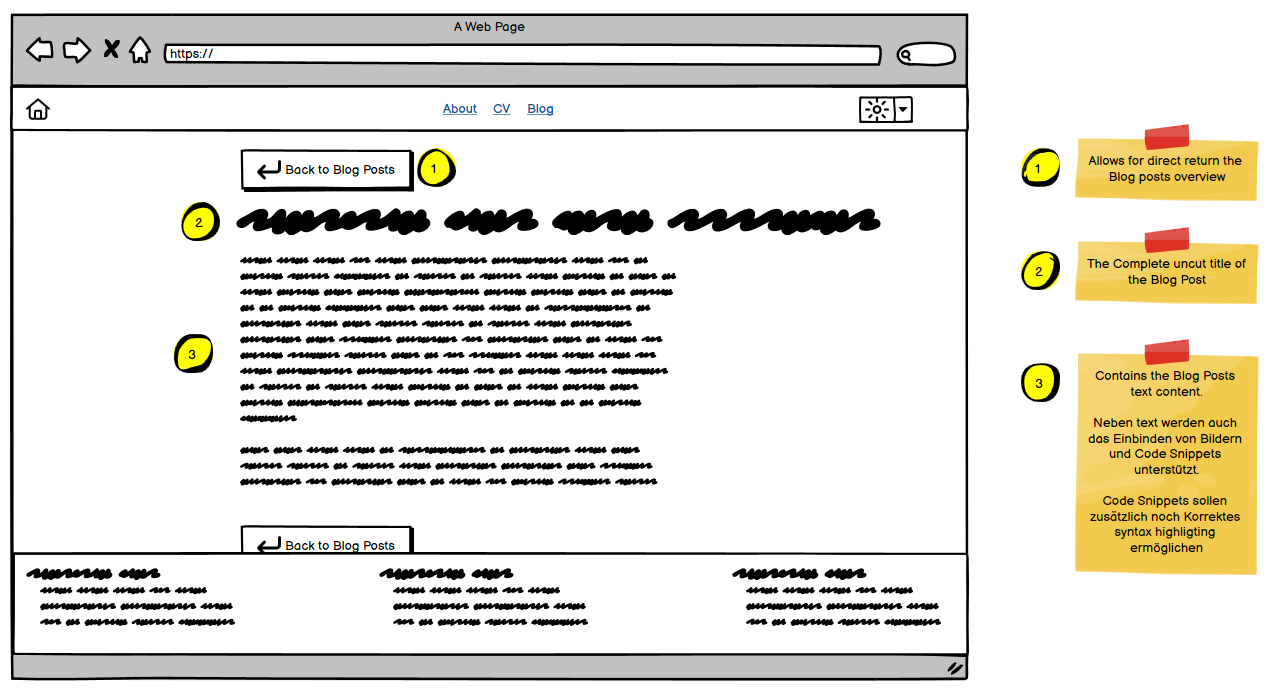
\includegraphics[width=0.5\textwidth]{blogentry.png}
    \\
    Quelle: Eigene Darstellung
\end{figure}


\newpage


\begin{landscape}
    \section{ Projektmanagement }
\subsection{ Anforderungsliste}
    % \begin{table}[H]
    %     \begin{tabular}{|l|l|l|l|l|l|}
    %     \hline
    %     \# & \textbf{System} & \textbf{Wichtigkeit} & \textbf{Art der Funktionaltität} & \textbf{Objekt} & \textbf{Funktionalität} \\ \hline
    %     1  &  Blog           &     Muss             &       Fähig sein                 &      Markdown   &  zu Parsen und Rendern  \\ \hline
    %     1  &  Blog           &     Muss             &       Fähig sein                 &      Code Snippets   &  zu Highlighten    \\ \hline
    %     1  &  Blog           &     Sollte             &     Die Möglichkeit bieten     &      Blog Einträge   &  zu filtern  \\ \hline
    %     1  &  Blog           &     sollte             &       ie Möglichkeit bieten    &    Blog Einträge   &   mit einem Cover Image hervor zu heben \\ \hline
    %     2  &  Blog           &     Muss              &       Fähig sein                &      Meta daten           &     anzuzeigen                    \\ \hline
    %     3  &                 &                      &                                  &                 &                         \\ \hline
    %     \end{tabular}
    %     \caption{Anforderungsliste}
    %     \label{tab:Anforderungsliste}
    % \end{table}

    \begin{table}[h!]
        \centering
        \begin{tabular}{|c|l|c|l|l|p{6cm}|}
        \hline
        \# & System    & Wichtigkeit & Art der Funktionalität       & Objekt           & Funktionalität                                                    \\ \hline
        1  & Blog      & Muss        & Markdown-Parsing             & Blog-Artikel     & Fähig sein, Markdown zu parsen und korrekt darzustellen.          \\ \hline
        2  & Blog      & Muss        & Syntax-Highlighting          & Code-Snippets    & Fähig sein, Code-Snippets in Artikeln hervorzuheben.              \\ \hline
        3  & Blog      & Sollte      & Filterfunktion               & Blog-Artikel     & Die Möglichkeit bieten, Blog-Einträge nach Kategorien zu filtern. \\ \hline
        4  & Blog      & Sollte      & Cover-Bild                   & Blog-Artikel     & Blog-Einträge mit einem Cover-Bild hervorheben können.            \\ \hline
        5  & Blog      & Muss        & Meta-Daten-Anzeige           & Blog-Artikel     & Fähig sein, Meta-Daten (Autor, Veröffentlichungsdatum) anzuzeigen.\\ \hline
        6  & Portfolio & Muss        & Lebenslauf                   & Portfolio-Seite  & Darstellung des Lebenslaufs und der beruflichen Erfahrungen.      \\ \hline
        7  & Portfolio & Muss        & Projektübersicht             & Portfolio-Seite  & Präsentation von abgeschlossenen Projekten mit detaillierten Beschreibungen. \\ \hline
        8  & CI/CD     & Muss        & Automatisierte Tests         & Gesamtsystem     & Automatische Ausführung von Tests bei jeder Änderung.             \\ \hline
        9  & CI/CD     & Muss        & Automatisierte Deployments   & Gesamtsystem     & Automatische Bereitstellung von Updates nach erfolgreichen Tests. \\ \hline
        10 & Website   & Muss        & Responsive Design            & Gesamtsystem     & Sicherstellen, dass die Webseite auf verschiedenen Geräten gut aussieht und funktioniert. \\ \hline
        11 & Website   & Sollte      & SEO-Optimierung              & Gesamtsystem     & Optimierung der Webseite für Suchmaschinen, um die Sichtbarkeit zu erhöhen. \\ \hline
        12 & Website   & Sollte      & Analytics-Integration        & Gesamtsystem     & Integration von Analysetools, um das Nutzerverhalten zu verfolgen und zu analysieren. \\ \hline
        \end{tabular}
        \caption{Anforderungsliste}
        \label{table:anforderungsliste}
        \end{table}

        
\end{landscape}


\begin{landscape}
    \subsection{ Risiken }
\begin{table}[h!]
    \centering
    \begin{tabular}{|c|l|p{6cm}|l|c|c|p{6cm}|}
    \hline
    \# & System      & Risiko                                                & Typ                & Wahrscheinlichkeit & Schwere  & Maßnahme                                                    \\ \hline
    1  & Blog        & Sicherheitslücken bei der Verarbeitung von Markdown   & Technisch          & Mittel             & Hoch     & Regelmäßige Sicherheitsupdates und Code-Reviews             \\ \hline
    2  & CI/CD       & Fehlgeschlagene Deployments                           & Technisch/Operativ & Mittel             & Mittel   & Automatisierte Tests und Rücksetzmechanismen (Rollback)     \\ \hline
    3  & Website     & Nicht optimierte Ladezeiten                           & Performance        & Hoch               & Mittel   & Implementierung von Caching und Code-Optimierung            \\ \hline
    4  & Portfolio   & Unvollständige oder veraltete Projektdaten            & Inhaltlich         & Mittel             & Mittel   & Regelmäßige Aktualisierung und Überprüfung der Inhalte      \\ \hline
    5  & Blog        & Datenverlust bei Artikelveröffentlichung              & Technisch          & Niedrig            & Hoch     & Regelmäßige Backups und Versionskontrolle                   \\ \hline
    6  & CI/CD       & Integration neuer Technologien ohne ausreichende Tests& Technisch          & Mittel             & Hoch     & Umfangreiche Testphase und schrittweise Integration         \\ \hline
    7  & Website     & Unzureichende SEO-Optimierung                         & Marketing          & Mittel             & Mittel   & Einsatz von SEO-Tools und regelmäßige SEO-Audits            \\ \hline
    8  & Website     & Inkompatibilität mit bestimmten Browsern oder Geräten & Technisch          & Mittel             & Mittel   & Umfangreiche Kompatibilitätstests und responsive Design     \\ \hline
    9  & Blog        & Mangelnde Nutzerakzeptanz für das Blogging-System     & Benutzerakzeptanz  & Niedrig            & Mittel   & Benutzerfreundliches Design und Feedbackmechanismen         \\ \hline
    10 & Portfolio   & Datenschutzverletzungen bei personenbezogenen Daten   & Rechtlich          & Niedrig            & Hoch     & Einhaltung von Datenschutzrichtlinien und -gesetzen         \\ \hline
    11 & CI/CD       & Überlastung der Server durch häufige Deployments      & Performance        & Niedrig            & Mittel   & Lasttests und Skalierungsstrategien                         \\ \hline
    12 & Website     & Unzureichende Barrierefreiheit                        & Technisch/Social   & Mittel             & Mittel   & Einhaltung von Barrierefreiheitsstandards und -richtlinien  \\ \hline
    \end{tabular}
    \caption{Risikoliste}
    \label{table:risikoliste}
    \end{table}
\end{landscape}
    

\subsection{ Projektressourcen }
\subsubsection{ Personen }
%Name Arbeitgeber Arbeitsumfeld Arbeitserfahrung

\begin{table}[H]
    \begin{tabular}{|l|l|l|l|l|}
        \hline
        \# & \textbf{Name}   & \textbf{Arbeitgeber} & \textbf{Arbeitsumfeld}           & \textbf{Arbeitserfahrung}        \\ \hline
        1  &  Johannes Lüke  &     Siemens AG       &    \makecell{ Softwareentwicklung\\Automatisierungstechnik  }   & <6 Jahre\\ \hline
    \end{tabular}
    \caption{Personen}
    \label{tab:Personen}
\end{table}

\subsubsection{ Projektteam }

\begin{table}[H]
    \begin{tabular}{|l|l|l|l|l|}
    \hline
    \# & \textbf{Arbeitskraft}   & \textbf{Funktion}    \\ \hline
    1  &  Johannes Lüke          &  Projektleiter       \\ \hline
    2  &  Johannes Lüke          &  Entwickler       \\ \hline
    3  &  Johannes Lüke          &  Architekt       \\ \hline
    4  &  Johannes Lüke          &  DevOps       \\ \hline 
    \end{tabular}
    \caption{Team/Rollen}
    \label{tab:TeamRollen}
\end{table}

\subsubsection{ Personalaufwand }

\begin{table}[H]
    \begin{tabular}{|l|l|l|l|}
    \hline
    \# & \textbf{Name}    & \textbf{Arbeitskraft} & \textbf{Effort (in Month)}        \\ \hline
    1  &  Projektplanung  &     Lüke              &          1              \\ \hline
    2  &  CI/CD           &     Lüke              &          1              \\ \hline
    3  &  Markdown        &     Lüke              &          1              \\ \hline
    4  &  Blog            &     Lüke              &          1              \\ \hline
    Summe  &              &                   &          4             \\ \hline
    \end{tabular}
    \caption{Aufwände in Personen Monaten}
    \label{tab:PersonenMonate}
\end{table}


\subsubsection{ Personalkosten }

\begin{table}[H]
    \begin{tabular}{|l|l|l|l|}
    \hline
    \# & \textbf{Arbeitskraft}    & \textbf{Kosten} & \textbf{ Kosten * Zeit }        \\ \hline
    1  &  Lüke          &     123 €/h     &          68.880 €             \\ \hline
   
    \end{tabular}
    \caption{Aufwände in Euro}
    \label{tab:Kosten}
\end{table}
 
\subsection{ Projektschätzungen }
Auf Grund des kleinen Teams wurde keine Projektschätzung durchgeführt, da der
entstehende Nutzen für den angestrebten Projektzeitraum in keinem guten Verhältnis steht.

\begin{landscape}
    \subsection{ Arbeitspackete}

    \begin{longtable}{|c|l|c|c|c|p{3cm}|p{3cm}|p{3cm}|}
        \hline
        \# & Titel                       & Start       & Ende        & Dauer (Wochen) & Ziel                                                                 & Arbeitsbeschreibung                                                      & Risiken                                                       \\ \hline
        1  & Projektplanung              & 01.03.2024  & 14.03.2024  & 2              & Strukturierte Planung und Vorbereitung des Projekts                  & Erstellen des Projektplans, Ressourcenplanung, Festlegung der Ziele und Meilensteine & Unklare Anforderungen, Verzögerungen durch unvollständige Planung   \\ \hline
        2  & Anforderungsanalyse         & 15.03.2024  & 28.03.2024  & 2              & Detaillierte Anforderungsermittlung und -dokumentation                & Interviews mit Stakeholdern, Erstellung der Anforderungsliste, Priorisierung der Anforderungen & Missverständnisse bei der Anforderungsermittlung, fehlende Stakeholder-Beteiligung \\ \hline
        3  & Architekturdesign           & 29.03.2024  & 11.04.2024  & 2              & Entwurf einer skalierbaren und robusten Architektur                   & Erstellung des Architekturdesigns, Auswahl der Technologien                        & Falsche Technologieentscheidungen, unvollständiges Design            \\ \hline
        4  & Implementierung             & 12.04.2024  & 09.05.2024  & 4              & Entwicklung der Kernfunktionalitäten der Webseite                     & Codierung der Webseite, Integration von CI/CD, Implementierung des Blog- und Portfolio-Systems & Technische Probleme, Verzögerungen bei der Implementierung           \\ \hline
        4.1 & Frontend-Entwicklung        & 12.04.2024  & 18.04.2024  & 1              & Erstellung des Benutzeroberfläche                                      & Entwicklung der Benutzeroberfläche mit Angular, Implementierung der Grundstruktur & Designprobleme, Benutzerfreundlichkeit                              \\ \hline
        4.2 & Blog-System                 & 19.04.2024  & 25.04.2024  & 1              & Implementierung des Blogging-Systems                                  & Entwicklung des Markdown-Parsers, Syntax-Highlighting für Code-Snippets              & Parsing-Fehler, Sicherheitslücken bei der Verarbeitung               \\ \hline
        4.3 & Portfolio-System            & 26.04.2024  & 02.05.2024  & 1              & Entwicklung des Portfolio-Systems                                      & Erstellung der Portfolio-Seiten, Implementierung der Projektübersicht                  & Unvollständige Daten, Probleme bei der Darstellung                   \\ \hline
        4.4 & CI/CD-Integration           & 03.05.2024  & 09.05.2024  & 1              & Integration der CI/CD-Pipeline                                         & Einrichtung automatisierter Tests und Deployments                                  & Fehlgeschlagene Deployments, unzureichende Testabdeckung             \\ \hline
        5  & Testing                      & 10.05.2024  & 23.05.2024  & 2              & Sicherstellung der Funktionalität und Qualität der Webseite            & Durchführung von Unit-Tests, Integrationstests und Systemtests                      & Unentdeckte Fehler, unzureichende Testabdeckung                       \\ \hline
        6  & Deployment                   & 24.05.2024  & 30.05.2024  & 1              & Erfolgreiche Bereitstellung der Webseite auf der Produktionsumgebung    & Vorbereitung der Deployment-Umgebung, Durchführung des Deployments, Überwachung     & Fehler beim Deployment, Ausfallzeiten während des Deployments        \\ \hline
        7  & Dokumentation                & 31.05.2024  & 13.06.2024  & 2              & Erstellung einer umfassenden Projektdokumentation                      & Schreiben von Benutzerhandbüchern, Entwicklerdokumentation und Projektberichten     & Unvollständige oder unklare Dokumentation                            \\ \hline
        8  & Review und Abschluss         & 14.06.2024  & 20.06.2024  & 1              & Projektbewertung und Abschluss                                         & Durchführung von Reviews, Erstellung des Abschlussberichts, Lessons Learned Session & Fehlende Beteiligung der Stakeholder, unvollständige Projektbewertung \\ \hline
        \caption{Arbeitspakete}
        \label{table:arbeitspakete}
    \end{longtable} 
\end{landscape}
    

% Please add the following required packages to your document preamble:
% \usepackage{multirow}

% \begin{Epics}[captiontest]
%     \epic["test",1]
% \end{Epics}

% \begin{table}[]
%     \begin{tabular}{|l|lllllllll|}
%         \hline
%         \textbf{Epic}                            & \multicolumn{7}{c|}{\textbf{Title}}                                                                                                                                               & \multicolumn{1}{l|}{\textbf{Effort}}        & 0        \\ \hline
%         \multicolumn{1}{|c|}{\multirow{4}{*}{0}} & \multicolumn{1}{l|}{\textbf{Feature}}   & \multicolumn{6}{c|}{\textbf{Title}}                                                                                                     & \multicolumn{1}{l|}{\textbf{Effort}}        & 0        \\ \cline{2-10} 
%         \multicolumn{1}{|c|}{}                   & \multicolumn{1}{c|}{\multirow{3}{*}{0}} & \multicolumn{1}{l|}{\textbf{Userstory}} & \multicolumn{5}{c|}{\textbf{Title}}                                                           & \multicolumn{1}{l|}{\textbf{Effort}}        & 0        \\ \cline{3-10} 
%         \multicolumn{1}{|c|}{}                   & \multicolumn{1}{c|}{}                   & \multicolumn{1}{c|}{\multirow{2}{*}{0}} & \multicolumn{1}{l|}{\textbf{Description}}         & \multicolumn{6}{l|}{As a Developer i want ...}                                                     \\ \cline{4-10} 
%         \multicolumn{1}{|c|}{}                   & \multicolumn{1}{c|}{}                   & \multicolumn{1}{c|}{}                   & \multicolumn{1}{l|}{\textbf{Acceptance Criteria}} & \multicolumn{6}{l|}{\begin{tabular}[c]{@{}l@{}}+ Unittest\\ + Linting\\ + Otherstuff\end{tabular}} \\ \hline
        
%         \textbf{Epic}                            & \multicolumn{7}{c|}{\textbf{title}}                                                                                                                                               & \multicolumn{1}{l|}{\textbf{Effort}}        & 0        \\ \hline
%         \multirow{7}{*}{1}                       & \multicolumn{1}{l|}{\textbf{Feature}}   & \multicolumn{6}{c|}{\textbf{title}}                                                                                                     & \multicolumn{1}{l|}{\textbf{Effort}}        & 0        \\ \cline{2-10} 
%                                                  & \multicolumn{1}{l|}{\multirow{6}{*}{0}} & \multicolumn{1}{l|}{\textbf{Userstory}} & \multicolumn{5}{c|}{\textbf{Title}}                                                           & \multicolumn{1}{l|}{\textbf{Effort}}        & 0        \\ \cline{3-10} 
%                                                  & \multicolumn{1}{l|}{}                   & \multicolumn{1}{l|}{\multirow{2}{*}{0}} & \multicolumn{1}{l|}{\textbf{Description}}         & \multicolumn{6}{l|}{As a Developer i want ...}                                                     \\ \cline{4-10} 
%                                                  & \multicolumn{1}{l|}{}                   & \multicolumn{1}{l|}{}                   & \multicolumn{1}{l|}{\textbf{Acceptance Criteria}} & \multicolumn{6}{l|}{\begin{tabular}[c]{@{}l@{}}+ Unittest\\ + Linting\\ + Otherstuff\end{tabular}} \\ \cline{3-10} 
%                                                  & \multicolumn{1}{l|}{}                   & \multicolumn{1}{l|}{\textbf{Userstory}} & \multicolumn{5}{c|}{\textbf{Title}}                                                           & \multicolumn{1}{l|}{\textbf{Effort}}        & 0        \\ \cline{3-10} 
%                                                  & \multicolumn{1}{l|}{}                   & \multicolumn{1}{l|}{\multirow{2}{*}{1}} & \multicolumn{1}{l|}{\textbf{Description}}         & \multicolumn{6}{l|}{}                                                                              \\ \cline{4-10} 
%                                                  & \multicolumn{1}{l|}{}                   & \multicolumn{1}{l|}{}                   & \multicolumn{1}{l|}{\textbf{Acceptance Criteria}} & \multicolumn{6}{l|}{}                                                                              \\ \hline
%         \end{tabular}
%         \caption{}
%         \label{tab:my-table}
% \end{table}
% \newpage

% \section{ Continous Integration / Delivery} 
% \subsection{ Platform }
% \subsubsection{ Continous Integration }
% \paragraph{ Github Action }
% \paragraph{ Testing }
% \subsubsection{ Continous Delivery }
% \paragraph{ Release }
% \paragraph{ Deployment }





